\documentclass[landscape, a4paper]{article}

%!Tex Root = ../main.tex

% ┌────────────┐
% │ Formatting │
% └────────────┘
\usepackage[english]{babel}
\usepackage[top=0cm,bottom=0cm,left=0cm,right=0cm]{geometry}
\usepackage[export]{adjustbox} % use c, l, r for images
\usepackage{csquotes}
\usepackage[parfill]{parskip}
\usepackage{fontspec}
% \usepackage{anyfontsize}
% \usepackage[]{enumitem}

% ┌──────┐
% │ Math │
% └──────┘
\usepackage{amssymb} % for black triangleright, https://tex.stackexchange.com/questions/570303/use-blacktriangleright-as-itemize-label
\usepackage{amsmath}
\usepackage{mathtools} % for \mathclap and 
\usepackage{breqn}

% ┌────────┐
% │ Tables │
% └────────┘
\usepackage{tabularray}
 % \UseTblrLibrary{diagbox}

% ┌────────┐
% │ Images │
% └────────┘
\usepackage{graphicx}
% \usepackage{float} % for the letter H
% \graphicspath{figures/}
\usepackage{subcaption}

% ┌────────┐
% │ Graphs │
% └────────┘
\usepackage{tikzit}
\usepackage{tikz}
\usetikzlibrary{backgrounds}
\usetikzlibrary{arrows}
\usetikzlibrary{shapes,shapes.geometric,shapes.misc}

% this style is applied by default to any tikzpicture included via \tikzfig
\tikzstyle{tikzfig}=[baseline=-0.25em,scale=0.5]

% these are dummy properties used by TikZiT, but ignored by LaTex
\pgfkeys{/tikz/tikzit fill/.initial=0}
\pgfkeys{/tikz/tikzit draw/.initial=0}
\pgfkeys{/tikz/tikzit shape/.initial=0}
\pgfkeys{/tikz/tikzit category/.initial=0}

% standard layers used in .tikz files
\pgfdeclarelayer{edgelayer}
\pgfdeclarelayer{nodelayer}
\pgfsetlayers{background,edgelayer,nodelayer,main}

% style for blank nodes
\tikzstyle{none}=[inner sep=0mm]

% include a .tikz file
\newcommand{\tikzfig}[1]{%
{\tikzstyle{every picture}=[tikzfig]
\IfFileExists{#1.tikz}
  {\input{#1.tikz}}
  {%
    \IfFileExists{./figures/#1.tikz}
      {\input{./figures/#1.tikz}}
      {\tikz[baseline=-0.5em]{\node[draw=red,font=\color{red},fill=red!10!white] {\textit{#1}};}}%
  }}%
}

% the same as \tikzfig, but in a {center} environment
\newcommand{\ctikzfig}[1]{%
\begin{center}\rm
  \tikzfig{#1}
\end{center}}

% fix strange self-loops, which are PGF/TikZ default
\tikzstyle{every loop}=[]


% ┌────────┐
% │ Citing │
% └────────┘
% \usepackage[style=authortitle]{biblatex}
% \addbibresource{./Graph_Theory.bib}
% \usepackage{cleveref}

% ┌──────────┐
% │ Diagrams │
% └──────────┘
% \usepackage{tikz}
% \usetikzlibrary{shadows, backgrounds} % , calc

% ┌──────────────────┐
% │ Multiple columns │
% └──────────────────┘
% \usepackage{multicol}

% ┌────────────────────┐
% │ Code hightligthing │
% └────────────────────┘
% \usepackage{minted}

% ┌────────────────────────┐
% │ Latex Programming Help │
% └────────────────────────┘
\usepackage{etoolbox}
\usepackage{xparse}
% https://tex.stackexchange.com/questions/358292/creating-a-subcounter-to-a-counter-i-created
\usepackage{chngcntr}

% ┌───────────────┐
% │ Pretty Boxes  │
% └───────────────┘
\usepackage{xcolor}
\usepackage{tcolorbox}
\tcbuselibrary{skins,theorems}

% ┌──────────────┐
% │ Pseudo Code  │
% └──────────────┘
\usepackage{pseudo}

% \usepackage{background}
\usepackage{gradient-text}
\usepackage{rotating}

% \newlength\mylen
% \setlength\mylen{\dimexpr\paperwidth/80\relax}
%
% \SetBgScale{1}
% \SetBgAngle{0}
% \SetBgColor{blue!30}
% \SetBgContents{\tikz{\draw[step=\mylen] (-.5\paperwidth,-.5\paperheight) grid (.5\paperwidth,.5\paperheight);}}

% ┌────────────┐
% │ Misc Tools │
% └────────────┘
\usepackage{lipsum}

%!Tex Root = ../main.tex

% ┌────────────┐
% │ Formatting │
% └────────────┘
% \setlength{\parskip}{0.4cm} % space between paragraphs, https://latexref.xyz/bs-par.html

% ┌───────┐
% │ Fonts │
% └───────┘
\usepackage{fontspec}
\newfontfamily\gyre{DejaVu Math TeX Gyre}
% colored bold
% \newcommand\alert[1]{\textcolor{SwitchColor}{\textbf{#1}}}
\newcommand\alert[1]{\textcolor{SwitchColor}{#1}}

% ┌──────────────┐
% │ Pseudo Code  │
% └──────────────┘
\newcounter{algorithm}
\setcounter{algorithm}{0}
\newtcbtheorem[use counter=algorithm]{algorithm}{\color{SecondaryColor}Algorithm}{pseudo/ruled}{alg}
% \newcommand{\ma}[1]{$\mathcal{#1}$}
% \renewcommand{\tt}[1]{{\small\texttt{#1}}}

% ┌────────┐
% │ Colors │
% └────────┘
\definecolor{PrimaryColor}{HTML}{800080}
\definecolor{PrimaryColorDimmed}{HTML}{D6D6F0}
\definecolor{SecondaryColor}{HTML}{006BB6}
\definecolor{SecondaryColorDimmed}{HTML}{E5F0F8}
\definecolor{SwitchColor}{named}{PrimaryColor}
\colorlet{BoxColor}{gray!10!white}

% ┌───────┐
% │ Links │
% └───────┘
\usepackage[allbordercolors=PrimaryColor, pdfborder={0 0 .2}]{hyperref}

% ┌─────────┐
% │ Mindmap │
% └─────────┘
\renewcommand{\labelitemi}{$\textcolor{SwitchColor}{\bullet}$}
\renewcommand{\labelitemii}{$\textcolor{SwitchColor}{\blacktriangleright}$}
\renewcommand{\labelitemiii}{$\textcolor{SwitchColor}{\blacksquare}$}

%!Tex Root = ../main.tex

% ┌─────────┐
% │ Mindmap │
% └─────────┘
\newlength{\leveldistance}
\setlength{\leveldistance}{25cm}

\newenvironment{edges}{\begin{pgfonlayer}{background}\draw [concept connection]}{;\end{pgfonlayer}}
\newcommand{\edge}[2]{(#1) edge (#2)}
\newcommand{\annotation}[2]{\path (#1) -- node[annotation, above, align=center, pos=0.03] {#2} (middle);}

\newenvironment{resettikz}{\pgfsetlayers{nodelayer,edgelayer}\tikzset{every node/.style={fill opacity=1.0, draw opacity=1.0, minimum size=0cm, inner sep=0pt}}}{}

\newenvironment{mindmap}{
	\begin{tikzpicture}[
			auto,
			huge mindmap,
			fill opacity=0.6,
			draw opacity=0.8,
			concept color = PrimaryColorDimmed,
			every annotation/.style={fill=BoxColor, draw=none, align=center, fill = BoxColor, text width = 2cm},
			grow cyclic,
			level 1/.append style = {
					concept color=SecondaryColorDimmed,
					level distance=\leveldistance,
					sibling angle=360/\the\tikznumberofchildren,
					% https://tex.stackexchange.com/questions/501240/trying-to-use-the-array-environment-inside-a-tikz-node-with-execute-at-begin-no
					execute at begin node=\definecolor{SwitchColor}{named}{SecondaryColor}\definecolor{SwitchColorDimmed}{named}{PrimaryColorDimmed},
				},
			level 2/.append style = {
					concept color=PrimaryColorDimmed,
					level distance=\leveldistance / 2,
					sibling angle=35,
					execute at begin node=\definecolor{SwitchColor}{named}{PrimaryColor}\definecolor{SwitchColorDimmed}{named}{SecondaryColorDimmed},
				},
			level 3/.append style = {
					concept color=SecondaryColorDimmed,
					level distance=\leveldistance / 3,
					execute at begin node=\definecolor{SwitchColor}{named}{SecondaryColor}\definecolor{SwitchColorDimmed}{named}{PrimaryColorDimmed},
				},
			level 4/.append style = {
					concept color=PrimaryColorDimmed,
					level distance=\leveldistance / 4,
					execute at begin node=\definecolor{SwitchColor}{named}{PrimaryColor}\definecolor{SwitchColorDimmed}{named}{SecondaryColorDimmed},
				},
			level 5/.append style = {
					concept color=SecondaryColorDimmed,
					level distance=\leveldistance / 5,
					execute at begin node=\definecolor{SwitchColor}{named}{SecondaryColor}\definecolor{SwitchColorDimmed}{named}{PrimaryColorDimmed},
				},
			level 6/.append style = {
					concept color=PrimaryColorDimmed,
					level distance=\leveldistance / 6,
					execute at begin node=\definecolor{SwitchColor}{named}{PrimaryColor}\definecolor{SwitchColorDimmed}{named}{SecondaryColorDimmed},
				},
			level 7/.append style = {
					concept color=SecondaryColorDimmed,
					level distance=\leveldistance / 7,
					execute at begin node=\definecolor{SwitchColor}{named}{SecondaryColor}\definecolor{SwitchColorDimmed}{named}{PrimaryColorDimmed},
				},
			level 8/.append style = {
					concept color=PrimaryColorDimmed,
					level distance=\leveldistance / 8,
					execute at begin node=\definecolor{SwitchColor}{named}{PrimaryColor}\definecolor{SwitchColorDimmed}{named}{SecondaryColorDimmed},
				},
			level 9/.append style = {
					concept color=SecondaryColorDimmed,
					level distance=\leveldistance / 9,
					execute at begin node=\definecolor{SwitchColor}{named}{SecondaryColor}\definecolor{SwitchColorDimmed}{named}{PrimaryColorDimmed},
				},
			concept connection/.append style = {
					color = BoxColor,
				},
		]
		}{
	\end{tikzpicture}
}

\newenvironment{mindmapcontent}{
	\begin{scope}[
			every node/.style = {concept, circular drop shadow}, % draw=none
			every child/.style={concept},
		]
		}{
		;\end{scope}
}

% ┌───────┐
% │ Boxes │
% └───────┘
\DeclareTotalTCBox{\inlinebox}{ s m }
{standard jigsaw,opacityback=0,colframe=SwitchColor,nobeforeafter,tcbox raise base,top=0mm,bottom=0mm,
	right=0mm,left=0mm,arc=0.1cm,boxsep=0.1cm}
{\IfBooleanTF{#1}%
	{\textcolor{PrimaryColor}{\setBold >\enspace\ignorespaces}#2}%
	{#2}}

\DeclareTotalTCBox{\inlineboxtwo}{ s m }
{standard jigsaw,opacityback=0,colframe=SwitchColorDimmed,nobeforeafter,tcbox raise base,top=0mm,bottom=0mm,
	right=0mm,left=0mm,arc=0.1cm,boxsep=0.1cm}
{\IfBooleanTF{#1}%
	{\textcolor{SwitchColorDimmed}{\setBold >\enspace\ignorespaces}#2}%
	{#2}}

% ┌──────────────────┐
% │ Case distinction │
% └──────────────────┘
% \newtoggle{absolute}
% % \toggletrue{absolute}
% \togglefalse{absolute}
% \newcommand{\lpathgraph}[1]{\iftoggle{absolute}{/home/areo/Documents/Studium/Summaries/x/}{./}#1}

% ┌───────┐
% │ Fixes │
% └───────┘
% https://tex.stackexchange.com/questions/89467/why-does-pdftex-hang-on-this-file
% \newcommand{\colon}{\mathrel{\mathop:}}

% ┌───────┐
% │ Paths │
% └───────┘
% \newcommand{\script}[2]{\href[page=#1]{}{\inlinebox{#2}}}
\newcommand{\script}[2]{\href{openpdf:/home/areo/Documents/Studium/Semester_1_Master/Hardware_Security_and_Trust/slides/Slides annotated/Hardware_Security_and_Trust_all_in_one.pdf:#1}{\inlinebox{#2}}}
\newcommand{\scripttwo}[2]{\href{openpdf:///home/areo/Documents/Studium/Semester_1_Master/Hardware_Security_and_Trust/slides/Slides annotated/bonus/12_Lecture_06Dec.pdf:#1}{\inlinebox{#2}}}
\newcommand{\videoeight}[2]{\href{https://youtu.be/YcHSlFjcndU?feature=shared&t=#1}{\inlineboxtwo{#2}}}
\newcommand{\videonine}[2]{\href{https://youtu.be/3dL-3EOIfJ8?si=l3OakqHOeCpnNayw&t=#1}{\inlineboxtwo{#2}}}
\newcommand{\videoten}[2]{\href{https://youtu.be/6oF737pa510?feature=shared&t=#1}{\inlineboxtwo{#2}}}
\newcommand{\videoeleven}[2]{\href{https://youtu.be/PJTqfzTIYJs?feature=shared&t=#1}{\inlineboxtwo{#2}}}
\newcommand{\videotwelve}[2]{\href{https://youtu.be/oDxAH7aO-Tk?feature=shared&t=#1}{\inlineboxtwo{#2}}}
\newcommand{\videothirteen}[2]{\href{https://youtu.be/3TkSXxe_Ty8?feature=shared&t=#1}{\inlineboxtwo{#2}}}
\newcommand{\videofourteen}[2]{\href{https://youtu.be/1Y3dZuJ0MHg?feature=shared&t=#1}{\inlineboxtwo{#2}}}


\begin{document}
\fontsize{3pt}{3pt}\selectfont

\begin{minipage}[t]{0.2\linewidth}
	\fbox{General} \lecturenotes{/home/areo/Documents/Studium/Semester_2_Master/Program_Verification/slides/bonus/1._Introduction.md} \additionalslides{/home/areo/Documents/Studium/Semester_2_Master/Program_Verification/slides/bonus/1._Introduction.pdf}
	\begin{betterlist}
		\item \alert{Program Verifier:} Takes program and specification and determines whether the program satisfies or if it violates the specification. Tells that in all executions of program specification holds. Also want indication of how specification is violated (i.e. counter example, e.g. inputs to violate assert statement) and also in case of yes want proof, because the program verifier itself could have a bug. \underline{Typical specifications:} No division by zero, Array only accessed within its bounds, Termination, Memory safety, No assert statement is violated
		\item \href{https://ultimate-pa.org/?ui=tool&tool=automizer}{Ultimate Automizer}
		\item \underline{Challenges:}
		\begin{enumerate}
			\item \alert{Undecidability:} The program verification problem is undecidable. There's no algorithm that verify the program and always hold (\underline{compromise:} verification algorithm that always tells correct resutl when it terminates but may not terminate or algorithm that sometimes terminates and says it could not prove the program). \underline{Solution:} Do not try to develop algorithms that solve the problem for all programs. Algorithms that solve the problem for some programs are also helpful.
			\item \alert{Ambiguities:} Different programming languages disagree what should happen for a piece of code. \underline{Solution:} Use mathematical logic to give programming languages a precise semantics
			\item \alert{Correctness Proofs are Hard to Find:} We cannot track all executions.
		\end{enumerate}
	\end{betterlist}
	\fbox{Propositional Logic (PL)} \lecturenotes{/home/areo/Documents/Studium/Semester_2_Master/Program_Verification/slides/bonus/2._Propositional_Logic.md} \additionalslides{/home/areo/Documents/Studium/Semester_2_Master/Program_Verification/slides/bonus/2._Propositional_Logic.pdf}
	\begin{betterlist}
		\item \script{29}{Syntax} and \script{31}{Semantics}, \script{32}{Examples}
		\begin{betterlist}
			\item \alert{Abbreviations:} $true := \neg false$, $(F_1 \lor F2 ) := \neg (\neg F_1 \land \neg F2)$, $(F_1 \rightarrow F2) := (\neg F_1 \lor F2)$, $(F_1 \leftrightarrow F2) := ((F_1 \rightarrow F2) \land (F2 \rightarrow F_1))$
			\item \underline{Terminology:} We call true, false \alert{atoms}, If $X \in V_{PL}$, we call $X$ an \alert{atom}, If $F$ is an atom, we call $F$ and $\neg F$ a \alert{literal}, We call the symbols $\neg$, $\wedge$, $\vee$, $\rightarrow$, $\leftrightarrow$ \alert{logical connectives}
			\item order of \alert{precedence} for logical connectives: $\neg, \land, \lor, \rightarrow, \leftrightarrow$. Binary operators are \alert{right-associative} ($F_1 \rightarrow F_2 \rightarrow F_3$ is $F_1 \rightarrow (F_2 \rightarrow F_3 )$)
		\end{betterlist}
		\item We call a PL formula $F$ \alert{satisfiable} if there is a variable assignment $\rho$ such that the evaluation $[[F]]_\rho$ is true. Otherwise, we say that $F$ is \alert{unsatisfiable}. We call a PL formula $F$ \alert{valid} if for all variable assignments $\rho$ the evaluation $[[F]]\rho$ is true
		\begin{betterlist}
			\item Deciding \alert{satisfiability} of a PL formula is an \alert{NP-complete} problem. \alert{Truth table} has problem of limited applicability, because a truth table has one row per variable assignment, and there are $2^n$ (exponential) variable assignments for $n$ variables. There are many algorithms that work well in practice and that are known to be \alert{polynomial} on relevant \alert{subclasses of PL formulas}. \alert{SAT solver} for propositional logic. \alert{SMT solver} (satisfiability modulo theories) for first order logic modulo theories
		\end{betterlist}
		\item Let $\Gamma = \{F_1, \ldots F_n\}$ be a set of PL formulas, and let $F'$ be another PL formula $F'$. We say that $\Gamma$ \alert{entails} $F'$ if for all variable assignments $\rho$ we have that if $[[F_i]]\rho = true$ holds for all $i \in \{1, \ldots n\}$, then also $[[F']]\rho = true$ holds. We use $\models$ to denote this entailment relation and we say that the entailment $\Gamma \models F'$ holds if $\Gamma$ entails $F'$. \script{38}{Examples}. Prove that $\{F_1, \ldots F_n\}$ entails $F'$:
		\begin{betterlist}
			\item truth table (Not doable if number of variables is high)
			\item prove that the PL formula $F_1 \land \ldots \land F_n \rightarrow F'$ is valid (Requires algorithm for checking validity)
			\item prove that the PL formula $\neg(F_1 \land . . . \land F_n \rightarrow F')$ is not satisfiable (Requires algorithm for checking satisfiability, implemented in SMT solvers)
			\begin{betterlist}
				\item the PL formula $F$ is valid iff the PL formula $\neg F$ is unsatisfiable. \script{39}{Proof}
			\end{betterlist}
			\item proof system
		\end{betterlist}
		\item We call two PL formulas $F_1$ and $F_2$ \alert{equivalent}, denoted $F_1 \equiv F_2$, if they evaluate to the same truth value under each variable assignment. $F_1 \equiv F_2 \text{iff} \{F_1\} \models F_2 \text{and} \{F_2\} \models F_1$
	\end{betterlist}
	\fbox{PL Proof system ($N_{PL}$)}
	\begin{betterlist}
		\item proof system for deriving valid PL entailments $\Gamma \models F$
		\item template for giving a proof. Reasoning according to a fixed number of rules. Prove once that every rule is \enquote{correct}. Check a proof $\leadsto$ check if every step is an instance of a rule. Find a proof $\leadsto$ find a sequence of rules
		\item $\mathcal{N}_{PL}$: Proof system for entailments between PL formulas. Proof rules are $(n + 1)$-ary relations over entailments denoted as: $\frac{\Gamma_1 \vDash F_1 \quad \ldots \quad \Gamma_n \vDash F_n}{\Gamma_{n+1} \vDash F_{n+1}}$.  If $\Gamma_i$ entails $F_i$ for all $i \in \{1, \ldots n\}$, then $\Gamma_{n+1}$ entails $F_{n+1}$
		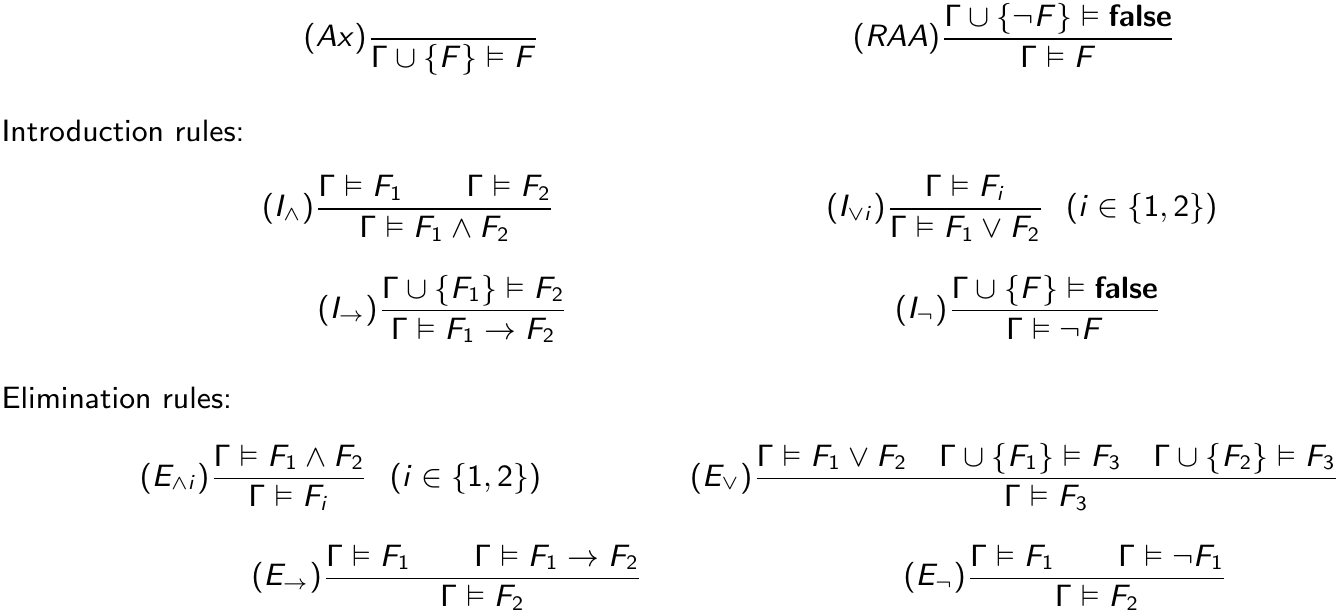
\includegraphics[width=0.7\linewidth]{./figures/proof_rules.png}  (called inference rules)
		\begin{betterlist}
			\item can find a derivation and conclude that the entailment holds
		\end{betterlist}
		\item A \alert{derivation} is a tree whose nodes are labelled by entailments such that the following holds: If a node labelled by entailment $\Gamma_{n+1} \models F_{n+1}$ has children that are labelled by entailments $\Gamma_1 ⊨ F_1 \ldots \Gamma_n ⊨ F_n$, then $\frac{\Gamma_1 \vDash F_1 \quad \ldots \quad \Gamma_n \vDash F_n}{\Gamma_{n+1} \vDash F_{n+1}}$ must be an instance of some rule. \script{44}{Example}. \script{45}{Remarks (f.)}
		\begin{betterlist}
			\item  \script{48}{Example: Construction of a Derivation}, \script{49}{Guide for proving entailments (f.)}
		\end{betterlist}
		\item \alert{Theorem (Soundness of $N_{PL}$):} If a node in a derivation is labelled by $\Gamma \models F$, then the entailment $\Gamma \models F$ holds. \script{47}{Proof}
		\item \alert{Theorem (Completeness of $N_{PL}$):} If the entailment $\Gamma \models F$ holds, then there exists a derivation where the root is labelled by $\Gamma \models F$
	\end{betterlist}
	\fbox{First-Order Logic (FOL)}
	\begin{betterlist}
		\item \script{56}{Examples (f.)}
		\item \underline{syntax:} \script{58}{Vocabulary and Terms}, \script{59}{Formulas}
		\begin{betterlist}
			\item $\forall x:\phi) := \neg(\exists x:\neg\phi)$, abbreviate $\exists x1 .\exists x2 .\phi$ to $\exists x1 , x2 .\phi$ and similarly for $\forall$
			\item \alert{quantifiers:}$\exists$ and $\forall$. \alert{atoms:} $true$, $false$, and $p(t_1, \ldots, t_n)$
			\item \alert{precedence} of quantifiers is lower than the precedence of logical connectives
			\item \script{60}{Model and $f \triangleleft \{\tilde{x}\rightarrow \tilde{y}\}$ notation}
			\item \underline{evaluation:} \script{61}{of terms} and \script{62}{of  formulas}
		\end{betterlist}
		\item we call a formula $\varphi$ \alert{satisfiable} if there exists a model $M$ and a variable assignment $\rho$ such that $[[\varphi]]_{M,\rho} = true$. Otherwise, $\varphi$ is \alert{unsatisfiable}. We call a formula $\varphi$ \alert{valid} if $[[\varphi]]_{M,\rho} = true$ for all models $M$ and for all variable assignments $\rho$
		\begin{betterlist}
			\item $\varphi$ is valid iff $\neg \varphi$ is unsatisfiable
		\end{betterlist}
		\item given a (possibly infinite) set of FOL formulas $\Gamma$ and a FOL formula $\psi$, we say that $\Gamma$ \alert{entails} $\psi$ if for all models $M$ and for all variable assignments $\rho$ we have that if $[[\phi]]_{M,\rho} = true$ holds for all $\phi \in \Gamma$ then also $[[\psi]]_{M,\rho} = true$ holds
		\begin{betterlist}
			\item we use $\models$ to denote this entailment relation and we say that \alert{the entailment $\Gamma \models \psi$ holds} if $\Gamma$ entails $\psi$
		\end{betterlist}
		\item \script{66}{Free Variables, Bound Variables, Closed Formulas}
		\item \script{67}{Substitution}
		\begin{betterlist}
			\item \underline{notation:}
			\begin{betterlist}
				\item given a function $f$, we use $dom(f)$ to denote the domain of $f$. Given a function $f$ that maps variables to terms, we use $vars(f)$ to denote the set that contains $dom(f)$ and all variables of all terms in the range of $f$. I.e., $\displaystyle vars(f) = dom(f) \cup \bigcup_{x\in dom(f)} freevars(f(x))$
				\item if we do not want to specify the substitution function $\sigma$ separately, we write $\varphi[x_1 \mapsto t_1, \ldots, x_n \mapsto t_n ]$ instead of $\varphi\sigma$ if $\sigma$ is the function that maps $x_i$ to $t_i$ for $i \in \{1, \ldots , n\}$.
				\item we sometimes use $\varphi[x]$ to refer to a formula and a variable. We may then use in this context $\varphi[t]$ to denote $\varphi[x \mapsto t]$
			\end{betterlist}
		\end{betterlist}
	\end{betterlist}
	\fbox{FOL Proof system ($N_{FOL}$)}
	\begin{betterlist}
		\item proof system for deriving valid FOL entailments $\Gamma \models \varphi$
		\item $N_{FOL}$ (natural deduction for first order logic):

		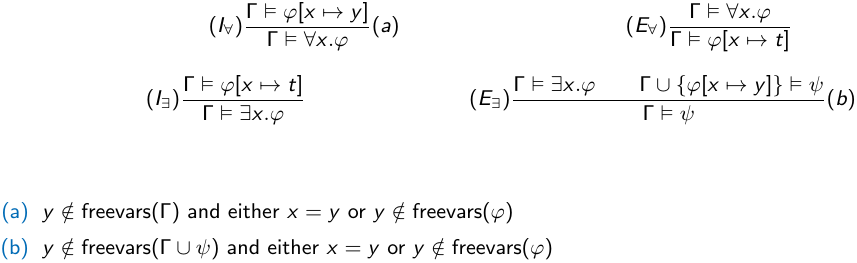
\includegraphics[width=0.7\linewidth]{./figures/nfol.png}
		\begin{betterlist}
			\item two of these rules have additional \alert{side conditions} that are written right beneath the rule. A tree is only a \textit{derivation} if all side conditions are satisfied. \script{72}{All rules}
		\end{betterlist}
		\item \underline{derivation:} \script{71}{Example}
		\begin{betterlist}
			\item use derivation (this tree) as a proof
		\end{betterlist}
		\item \script{80}{When use infix notation}
	\end{betterlist}
	\fbox{First-Order Theories}
	\begin{betterlist}
		\item \script{81}{Motivation (pr.)}
		\item \alert{first-order theory T} consists of:
		\begin{betterlist}
			\item a signature $\Sigma$ - set of constant, function, and predicate symbols
			\item a set of axioms $A_T$ - set of closed (no free variables) $\Sigma$-formulae
		\end{betterlist}
		\item a \alert{$\Sigma$-formula} is a formula constructed of constants, functions, and predicate symbols from $\Sigma$, and variables, logical connectives, and quantifiers
		\item \underline{idea:} the symbols of $\Sigma$ are just symbols without prior meaning. The axioms of $T$ provide their meaning
		\item \alert{$T$-model:} a model $M$ is a \alert{$T$ -model}, if $[[\varphi]]_{M,\rho} = true$ for all $\varphi \in A_T$ and for all variable assignments $\rho$
		\item \alert{$T$-valid:} a $\Sigma$-formula $\varphi$ is \alert{valid in theory $T$} (\alert{$T$ -valid}), if for every $T$ -model $M$ and variable assignment $\rho$, it holds that $[[\varphi]]_{M,\rho} = true$
		\item \alert{$T$-satisfiable:} a $\Sigma$-formula $\varphi$ is \alert{satisfiable} in $T$ (\alert{$T$ -satisfiable}), if there is a $T$ -model $M$ and variable assignment $\rho$ such that $[[\varphi]]_{M,\rho} = true$
		\item \alert{$T$-equivalent:} two $\Sigma$-formulae $\varphi_1$ and $\varphi_2$ are \alert{equivalent in $T$} (\alert{$T$ -equivalent}), if $\varphi_1 \leftrightarrow \varphi_2$ is $T$ -valid
		\item \script{90}{\alert{Axiom Schemata}}
	\end{betterlist}
\end{minipage}
\begin{minipage}[t]{0.2\linewidth}
	\fbox{Collection of First-Order Theories and their decidability} \lecturenotes{/home/areo/Documents/Studium/Semester_2_Master/Program_Verification/slides/bonus/06._First_Order_Theories.md} \additionalslides{/home/areo/Documents/Studium/Semester_2_Master/Program_Verification/slides/bonus/06._First_Order_Theories.pdf}
	\begin{betterlist}
		\item \script{89}{Theory of Equality (pr.)}, \script{93}{Theory of Rock-Paper-Scissors (pr.)}
		\item \alert{Decidability}: We call a problem \alert{decidable} if there exists an algorithm that terminates on all instances of the problem and gives a correct yes/no answer.
		\begin{betterlist}
			\item \uline{example undecidable problem:} Halting Problem for Turing machines, \uline{prove decidability:} give an algorithm and prove its correctness, \uline{prove undecidability:} reduction from a known undecidable problem
			\item \alert{Satisfiability} of PL formulas is \alert{decidable}, \alert{Satisfiability} of FOL formulas is \alert{undecidable}
			\item \alert{$T_{E}$-validity} is \alert{undecidable}, For a \alert{quantifier-free formula $T_E$-validity} is \alert{decidable}
			\item \script{100}{Peano Arithmetic $T_{PA}$ (first-order arithmetic) (ff.)}: natural numbers with addition and multiplication
			\begin{betterlist}
				\item \script{101}{Definition of $\le$ etc.}, \script{102}{$EXP[x, n, r]$}
				\item \alert{$T_{PA}$} is \alert{undecidable}, \alert{quantifier-free fragment of $T_{PA}$} is \alert{undecidable}
				\item \script{103}{\alert{Gödel’s first incompleteness theorem}}: \uline{Peano arithmetic $T_{PA}$ does not capture true arithmetic:} There exist closed $\Sigma_{PA}$-formulae representing valid propositions of number theory that are not $T_{PA}$-valid. \uline{The reason:} $T_{PA}$ actually admits nonstandard interpretations. \underline{For decidability:} \alert{no multiplication}
			\end{betterlist}

			\item \script{104}{Presburger Arithmetic $T_{\mathbb{N}}$}: natural numbers with addition
			\begin{betterlist}
				\item \alert{$T_{\mathbb{N}}$-satisfiability} and \alert{$T_{\mathbb{N}}$-validity} are \alert{decidable}
			\end{betterlist}
			\item \script{106}{Theory of Integers $T_{\mathbb{Z}}$ (pr.)}: integers with $+$, $−$, $>$
			\begin{betterlist}
				\item \alert{$T_{\mathbb{Z}}$-satisfiability} and \alert{$T_{\mathbb{Z}}$-validity} are \alert{decidable}
			\end{betterlist}
			\item \script{108}{Theory of Arrays $T^=_A$ (with extensionality)}, \script{109}{Theory of Bit-vectors (f.)}, \script{111}{Theory of Floats}
			\item \script{113}{Overview decidability}
		\end{betterlist}
	\end{betterlist}
	\fbox{SMT-LIB} \lecturenotes{/home/areo/Documents/Studium/Semester_2_Master/Program_Verification/slides/bonus/07._Boogie_and_Boostan.md} \additionalslides{/home/areo/Documents/Studium/Semester_2_Master/Program_Verification/slides/bonus/07._Boogie_and_Boostan.pdf}
	\begin{betterlist}
		\item \script{117}{What it is}, \script{118}{SMT Script}, \script{119}{Theories}, \script{122}{Logics (f.)}
		\item \script{124}{Terms definined in lecture and SMT-LIB (pr.)}, \script{126}{Terms (pr.)}
		\item \script{127}{Links to solvers}
		\item \script{129}{Commands (pr.)}
	\end{betterlist}
	\fbox{Boogie and Boostan Syntax}
	\begin{betterlist}
		\item \script{138}{Boogie and Boogaloo (prr.)}, \script{139}{Examples (f.)}, \script{141}{Options}
		\item \script{142}{Boostan}
		\item \script{146}{Context-free grammar}, \script{147}{Derivation tree}, \script{148}{Derived word}
		\item \script{152}{Grammar for Numbers}, \script{153}{Grammar for Variables}, \script{154}{Grammar for Integer Expressions}, \script{156}{Grammar for Boolean Expressions}, \script{157}{Grammar for Statements}
		\begin{betterlist}
			\item \underline{we call}: A subword that is derived from $X_{var}$ a (program) \alert{variable}, A subword that is derived from $X_{iexpr}$ or $X_{bexpr}$ an \alert{expression}, A subword that is derived from $X_{stmt}$ a (program) \alert{statement}
		\end{betterlist}
	\end{betterlist}
	\fbox{(Boogie and) Boostan Semantics}
	\begin{betterlist}
		\item \script{159}{Boostan program}
		\item \script{161}{Problem with C Semantics (ff.)}
		\item \script{167}{Relational semantics (f.)}
		\item \script{169}{Program State}, \script{179}{Set of states} (\script{170}{Sets of Program States (first mentioned)})
		\item \script{171}{Semantics of Expressions}
		\begin{betterlist}
			\item \underline{idea:} Assign each expression an SMT formula. Given an expression $expr$, we define the semantics of the expression, denoted $[[expr]]$ as the SMT formula that is denoted by the same string
			\item \script{171}{Exceptions}
			\item \script{179}{Convention: Omit double brackets} (\script{171}{Convention $expr$ instead of $[[expr]]$} (first mentioned))
		\end{betterlist}
		\item \script{172}{Semantics of the Assignment Statement (f.)}
		\item \script{178}{Semantics of the Concatenation of Statements}
		\begin{betterlist}
			\item \script{177}{Relational Composition}
		\end{betterlist}
		\item \script{180}{Semantics of the If-then-else Statement}
		\item \script{183}{Semantics of the While Statement}
		\begin{betterlist}
			\item \script{181}{Reflexive Transitive Closure} and \script{182}{Example}
		\end{betterlist}
		\item \script{184}{Full Example (f.)}
	\end{betterlist}
	\fbox{Hoare Proof System}
	\begin{betterlist}
		\item proof system for deriving valid Hoare triples $\{\varphi\} st \{\psi\}$
		\item a program $P$ \alert{satisfies the precondition-postcondition pair} $(\{\varphi_{pre}\}, \{\varphi_{post}\})$ if the inclusion $post(\{\varphi_{pre}\}, [[st]]) \subseteq \{\varphi_{post}\}$ holds (\script{189}{Precondition-Postcondition Pairs})
		\begin{betterlist}
			\item given a binary relation $R$ over the set $X$ and a subset of $Y \subseteq X$, the \alert{postimage of $Y$ under $R$},
			denoted $post(Y , R)$, is the set $\{x \in X \mid \text{ exists } y \in Y \text{ such that } (y, x) \in R\}$. \script{190}{Example}
			\item \script{191}{Full Example}
		\end{betterlist}
		\item given a set of states $\{\varphi\}$, a program statement $st$ and a set of states $\{\psi\}$, we call the triple $\{\varphi\} st \{\psi\}$ a \alert{Hoare triple}
		\item we call a Hoare triple $\{\varphi\} st \{\psi\}$ \alert{valid} if $st$ satisfies the precondition-postcondition pair $(\{\varphi\}, \{\psi\})$. \script{197}{Example}
		\item \underline{\script{200}{Rules}:}

		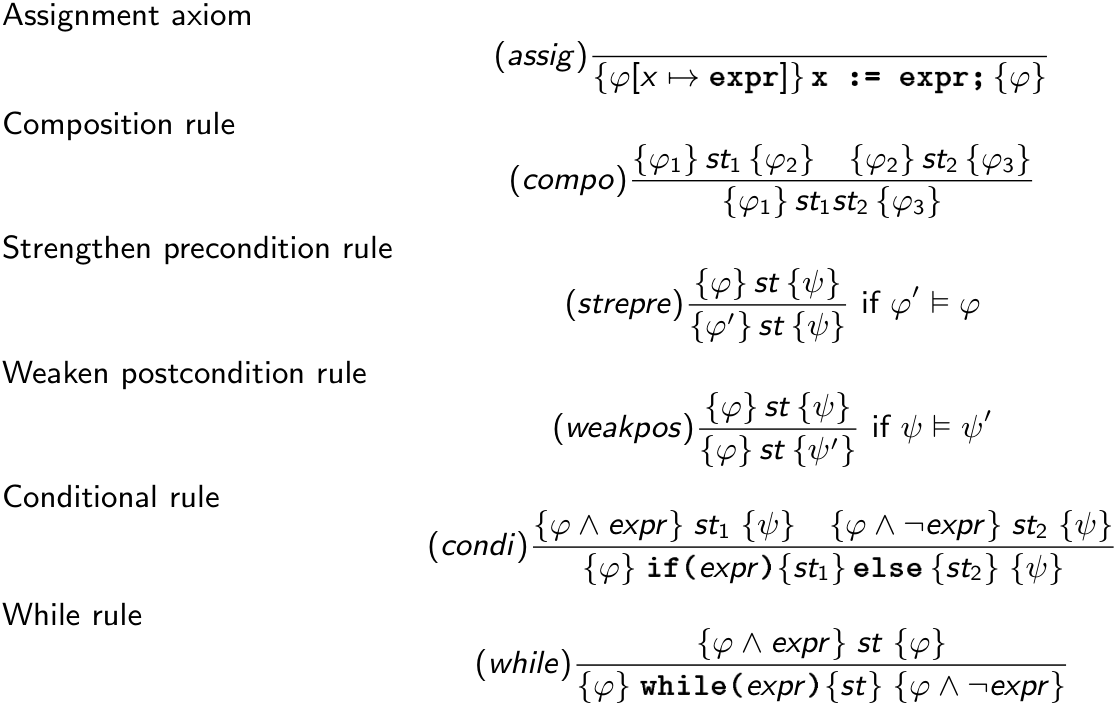
\includegraphics[width=0.7\linewidth]{./figures/hoare_rules.png}
		\begin{betterlist}
			\item \script{202}{Example: Assignment axiom}
			\item \script{203}{Example: Conditional Rule}
			\item \script{204}{Example: While Rule}
			\item \script{205}{Full Example}
		\end{betterlist}
		\item we define a \alert{derivation} as a tree whose nodes are labelled by Hoare triples such that the following holds. If a node that is labelled by a Hoare triple $\{\varphi_{n+1}\} st_{n+1} \{\psi_{n+1}\}$ has children that are labelled by Hoare triples $\{\varphi_1\} st_1 \{\psi_1\} \ldots \{\varphi_n\} st_n \{\psi_n\}$, then the following must be an instance of some rule: $\frac{\{\varphi_1\} st_1 \{\psi_1\} \ldots \{\varphi_n\} st_n \{\psi_n\}}{\{\varphi_{n+1}\} st_{n+1} \{\psi_{n+1}\}}$ (\script{201}{Derivation in context hoare proof system})
		\item \alert{Soundness of the Hoare Proof System:} If there is a derivation whose root is labelled by $\{\varphi\} st \{\psi\}$, then the statement $st$ satisfies the precondition-postcondition pair $(\{\varphi\}, \{\psi\})$
		\begin{betterlist}
			\item we call a rule of the form $\frac{\{\varphi_{1}\} st_{1} \{\psi_{1}\} \ldots \{\varphi_{n}\} st_{n} \{\psi_{n}\}}{\{\varphi_{n+1}\} st_{n+1} \{\psi_{n+1}\}}$ \alert{sound} if the following holds: If for all $i \in\{1, \ldots, n\}$ the Hoare triple ${\varphi_i} st_i {\psi_i}$ is valid, then the Hoare triple ${\varphi_{n+1}} st_{n+1} {\psi_{n+1}}$ is also valid. (\script{209}{Sound rule})
			\item \script{210}{Soundness of the Assignment Axiom}
			\item \script{211}{Soundness of the Composition Rule}
			\item \script{212}{Soundness of the Strengthen Precondition Rule}
			\item \script{213}{Soundness of the Weakening Postcondition Rule}
			\item \script{214}{Soundness of the Conditional Rule}
			\item \script{215}{Soundness of the While Rule (ff.)}
			\item \script{218}{Soundness of the Hoare Proof System (f.)}
		\end{betterlist}
	\end{betterlist}
	\fbox{Boostan Extended Syntax}
	\begin{betterlist}
		\item \script{242}{Arrays}
		\begin{betterlist}
			\item \script{243}{SMT-LIB}
			\item \script{244}{Memory via Arrays}
			\item \script{249}{Grammar}
		\end{betterlist}
		\item \script{255}{Havoc Statement (f.)}
		\begin{betterlist}
			\item \href{https://www.microsoft.com/en-us/research/wp-content/uploads/2016/12/krml178.pdf}{\inlinebox{Section 9.4 of Specification}}
			\item \script{258}{Grammar}
		\end{betterlist}
		\item \script{264}{Assume Statement}
		\begin{betterlist}
			\item \href{https://www.microsoft.com/en-us/research/wp-content/uploads/2016/12/krml178.pdf}{\inlinebox{Section 9.2 of Specification}}
			\item \script{266}{Grammar}
		\end{betterlist}
		\item Assert Statement
		\begin{betterlist}
			\item \script{436}{Grammar}
		\end{betterlist}

	\end{betterlist}
	\fbox{Boostan Extended Semantics}
	\begin{betterlist}
		\item \script{250}{Arrays}
		\item \script{259}{Havoc Statement}
		\item \script{267}{Assume Statement}
	\end{betterlist}
	\fbox{Hoare Proof System Extended}
	\begin{betterlist}
		\item \underline{Rules:}

		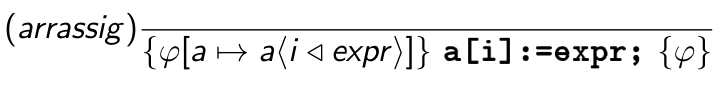
\includegraphics[width=0.5\linewidth]{./figures/arrassig.png}

		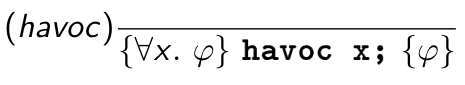
\includegraphics[width=0.325\linewidth]{./figures/havoc.png}

		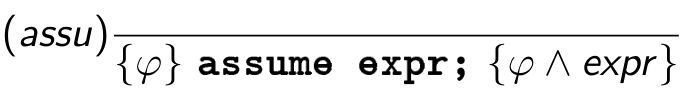
\includegraphics[width=0.4\linewidth]{./figures/assu.png}
		\begin{betterlist}
			\item \script{252}{Soundness of the Array Assignment Axiom}
			\item \script{261}{Soundness of the Havoc Axiom}
			\item \script{269}{Soundness of the Assume Axiom}
		\end{betterlist}
	\end{betterlist}
\end{minipage}
\begin{minipage}[t]{0.2\linewidth}
	\fbox{Ultimate Referee}
	\begin{betterlist}
		\item \script{227}{Guide for Finding a Derivation in the Hoare Proof System}
		\item \script{230}{What it is and example (ff.)}
		\item \script{233}{Interactive verification, Deductive verification, Automated verification}
	\end{betterlist}
	\fbox{Control-flow graphs}
	\begin{betterlist}
		\item \script{279}{Control-Flow Graph}, \script{279}{Control-Flow Graph for a Program}, \script{280}{Example}
		\begin{betterlist}
			\item \underline{useful for automated verification:} apply algorithms from graph theory / automata theory
			\item captures only one aspect of a program, it defines the way in which the programmer arranged the statements in the code
			\item focused solely on the program’s data but it is not sufficient to specify the situation in which a program currently is, because the state does not provide information about the next statements that can be executed
			\item \script{281}{Notational Conventions}
			\item all control-flow graphs for a given statement are \alert{isomorphic} to each other
		\end{betterlist}
		\item \script{282}{Sequential Composition}, \script{283}{Example}
		\item \script{284}{Conditional Statement}, \script{285}{Example}
		\item \script{286}{While Statement}, \script{287}{Example}
		\item we call a pair $(\ell, s)$ a \alert{program configuration} of $P$ if $\ell \in Loc$ is a location and $s$ is a state of $P$
		\item we call a sequence of program configurations $(\ell_0, s_0), . . . , (\ell_n, s_n)$ an \alert{execution} of $P$ if there exists a sequence of statements $st_1 \ldots st_n$ such that for each $i \in \{0, \ldots, n−1\}:$ $(\ell_i, st_{i+1}, \ell_{i+1}) \in \Delta$and $(s_i, s_{i+1}) \in [[st_{i+1}]]$. \script{292}{Example}
		\begin{betterlist}
			\item Executions do not have to start at the initial location and do not have to end at the exit location
		\end{betterlist}
		\item we call the program configuration $(\ell, s)$
		\begin{betterlist}
			\item \alert{initial}, if $\ell= \ell_{init}$ and $s \in\{\varphi_{pre}\}$
			\item an \alert{error configuration} if $\ell= \ell_{ex}$ and $s \not\in \{\varphi_{post}\}$
		\end{betterlist}
		\item \alert{Theorem PppSatAndExec:} The program $P = (V, \mu, st)$ satisfies the precondition-postcondition pair $(\varphi_{pre}, \varphi_{post})$ iff there exists no execution $(\ell_0, s_0), \ldots, (\ell_n, s_n)$ such that $(\ell_0, s0)$ is an initial configuration and $(\ell_n, sn)$ is an error configuration
		\begin{betterlist}
			\item so far we only had one way to formally show that $(\varphi_{pre}, \varphi_{post})$ is not satisfied: compute the binary relation over states for this program to check if every pair satisfies the precondition-postcondition pair. By Theorem PppSatAndExec we now have an alternative within our formal setting: we can give an execution
			\item \script{296}{Example program that shows need for Theorem CorrectIffNoErrorReach}
			\item \underline{Proof via lemma \alert{RelAndExec}:} Let $G = (Loc, \Delta, \ell_{init}, \ell_{ex})$ be a control-flow graph for $st$, then there exists a program execution $(\ell_0, s_0), . . . , (\ell_n, s_n)$ with $\ell_0 = \ell_{init}$ and $\ell_n = \ell_{ex}$, iff $(s_0, s_n) \in [[st]]$
			\begin{betterlist}
				\item Proof by induction over the height of st’s derivation tree. Using the following five lemmas, the proof can be carried out analogously to the soundness proof for the Hoare proof system:
				\begin{betterlist}
					\item \script{303}{Single assignment, array, havoc or assume statement}
					\item \script{304}{Sequential composition of statements}
					\item \script{305}{Conditional statement}
					\item \script{306}{While Statement (ff.)}
				\end{betterlist}
			\end{betterlist}
			\item The theorem Theorem PppSatAndExec follows directly from 1) the lemma Lemma RelAndExec, 2) the definition of an error configuration, and 3) the definition of satisfiability of precondition-postcondition pairs
		\end{betterlist}
		\item \alert{Reachable Program Configuration:} We call a configuration $(\ell, s)$ \alert{reachable} if there exists a program execution $(\ell_0, s_0), . . . , (\ell_n, s_n)$ such that $(\ell_0, s_0)$ is an initial configuration and $(\ell_n, s_n) = (\ell, s)$
		\item \alert{Theorem CorrectIffNoErrorReach:} A program satisfies a given precondition-postcondition pair iff the set of reachable configurations does not contain an error configuration
		\item the \alert{set of reachable configurations $RC$} is the smallest set such that
		\begin{betterlist}
			\item each initial configuration is an element of RC
			\item if $(\ell, s) \in RC$, $(\ell, st, \ell') \in \Delta$ and $(s, s') \in [[st]]$ then $(\ell', s') \in RC$
		\end{betterlist}
		\item the \alert{reachability graph} is a pair $(RC, T)$ such that $((\ell, s), st, (\ell', s')) \in T$ iff $(\ell, st, \ell') \in \Delta$ and $(s, s') \in [[st]]$
		\begin{betterlist}
			\item \script{362}{Algorithm}
		\end{betterlist}
		\item \alert{Timestamps:} Each thread maintains a timestamp, We represent a timestamp as a natural number, Each time we process an event we increase the thread’s timestamp, Initially, the timestamp for each thread is $1$
		\begin{betterlist}
			\item \script{111}{Example}
		\end{betterlist}
	\end{betterlist}
	\fbox{Predicate Transformers}
	\begin{betterlist}
		\item main means for analyzing the effect of statements in the control-flow graph-based view on programs
		\item execute a loop-free program symbolically (i.e., on all inputs in parallel). Set of all states that are reachable after each of the statements. User formulas whose satisfying variable assignments are exactly the reachable sets of states. Define the strongest post predicate transfomer which allows to compute these formulas
		\item \alert{Strongest Postcondition:} Given a set of states $S$ and a statement $st$ the strongest postcondition is the post image of $S$ under the relation $[[st]]$, i.e. $sp(S, st) = post(S, [[st]])$
		\begin{betterlist}
			\item \underline{Idea:} Given a set of states $S$ and a statement \verb|st|, the strongest postcondition $sp(S, \verb|st|)$ is the set of states for which the following holds. If there is a state $s \in S$
			\begin{betterlist}
				\item in which we can execute \verb|st|,
				\item in which \verb|st| terminates, and
				\item $s'$ is a successor after executing \verb|st|
			\end{betterlist}
			then $s' \in sp(S, \verb|st|)$
			\item \alert{Assignment Statement:} $sp(\{\varphi\}, \verb|x := expr;| )$ is $\{\exists \hat x:\varphi[x \mapsto \hat x] \land x = expr[x \mapsto \hat x]\}$. \script{332}{Proof} and \script{333}{Example}
			\item \alert{Havoc Statement:} $sp(\{\varphi\}, \verb|havoc x;| )$ is $\{\exists x:\varphi\}$. \script{334}{Proof idea}
			\item \alert{Assume Statement:} $sp(\{\varphi\}, \verb|assume expr;| )$ is $\{\varphi \land expr\}$. \script{335}{Proof}
			\item \alert{Sequential Composition:} If $st$ is an sequential composition of the form $st_1st_2$, then $sp(S, st)$ is $sp(sp(S, st_1), st_2)$. \script{336}{Proof}
			\item \alert{Conditional Statement:} $sp(\{\varphi\}, \verb|if (expr) { st1 } else { st2 }|)$ is $sp(sp(S, \verb|assume expr;|), \verb|st1|)\cup sp(sp(S, \verb|assume !expr;|), \verb|st2|)$
			\item In general, we cannot express the strongest post of the \alert{while statement} as a formula
			\begin{betterlist}
				\item If \verb|st| is a while statement of the form \verb|while(expr){st}| then $sp(S, \verb|st|)$ is $\displaystyle \bigcup_{k\in \mathbb{N}} sp(sp^k(S, \verb|assume expr; st|), \verb|assume !expr;| )$
				\begin{betterlist}
					\item \uline{$k$-th iterative application application of the strongest post operator:}\\ $s p^k(S, s t)= \begin{cases}S & \text { if } k=0 \\ s p\left(s p^{k-1}(S, s t), s t\right) & \text { if } k>0\end{cases}$
				\end{betterlist}
				\item There are \script{340}{examples} in which the strongest post of a while statement can be expressed by a formula
			\end{betterlist}
			\item \script{318}{Example 1} and \script{338}{Example 2}
		\end{betterlist}
		\item \alert{Quantifier Elimination:} finding an equivalent quanfitier-free formula for a given formula
		\begin{betterlist}
			\item \alert{Destructive Equality Resolution 1:} If the variable $x$ does not occur in the term $t$ then the formula $\exists x:\varphi \land x = t$ and the formula $\varphi[x \mapsto t]$ are equivalent. \script{328}{Example and proof idea}
			\item \alert{Destructive Equality Resolution 2:} If the variable $x$ does not occur in the term $t$ then the formula $\forall x:\varphi \lor x \ne t$ and the formula $\varphi[x\mapsto t]$ are equivalent. \script{329}{Proof idea}
		\end{betterlist}
		\item Let $st$ be a statement, and let $\varphi$, $\psi$ be formulas. The following statements are equivalent:
		\begin{betterlist}
			\item $\{\varphi\} st \{\psi\}$ is a valid Hoare triple
			\item $sp(\{\varphi\}, st) \subseteq \{\psi\}$
			\item $\{\varphi\} \subseteq wp(\{\psi\}, st)$
		\end{betterlist}
	\end{betterlist}
	\fbox{Bounded Model Checking}
	\begin{betterlist}
		\item an \alert{abstract (program) configuration} is a pair $(\ell, \{\varphi\})$ where $\ell$ is a location and $\varphi$ is a formula over the program’s variables
		\item an \alert{abstract reachability graph} is a graph $(AC, T)$ where AC is a set of abstract configurations and $T ⊆AC × Stmt × AC$, such that
		\begin{enumerate}
			\item for each edge $((\ell, {\varphi}), st, (\ell', \{\varphi'\})) \in T$, we have $(\ell, st, \ell') \in \Delta$ and $sp(\{\varphi\}, st) \subseteq \{\varphi'\}$,
			\item for each abstract configuration $(\ell, \{\varphi\}) \in AC$ with $\varphi\not\equiv false$ and $(\ell, st, \ell') \in ∆$, there exists an abstract configuration $(\ell', \{\varphi'\}) \in AC$ such that $((\ell, \{\varphi\}), st, (\ell', \{\varphi'\})) \in T$,
			\item there exists $(\ell_{init}, \{\varphi_{init}\}) \in AC$ with $\{\varphi_{pre}\} \subseteq \{\varphi_{init}\}$, and
			\item for each abstract configuration $(\ell, \{\varphi\}) \in AC$ there is a path from $(\ell_{init}, \{\varphi_{init}\})$ to $(\ell, \{\varphi\})$, using edges in $T$
		\end{enumerate}
		\begin{betterlist}
			\item we call an abstract reachability graph for G a \alert{safety proof} if is does not contain an abstract error configuration
			\begin{betterlist}
				\item \script{372}{Example}
			\end{betterlist}
		\end{betterlist}
		\item a \alert{precise abstract reachability graph} is an abstract reachability graph $(AC, T)$ such that for each edge $((\ell, \{\varphi\}), st, (\ell', \{\varphi'\}))$ the equality $sp(\{\varphi\}, st) = \{\varphi'\}$ holds, and $\{\varphi_{init}\} = \{\varphi_{pre}\}$
		\begin{betterlist}
			\item a precise abstract reachability graph for a given control-flow graph is unique up to the formulas that represent the set of states at each location
			\item \script{354}{Example: Implementation of the GCD (pr.)}. None of the three tests shows a violation of the postcondition. If one starts to build the precise abstract reachability graph, one sees after a few iterations that there is an abstract program configuration whose set of states is not a subset of the postcondition
			\item \script{363}{Algorithm}
			\begin{betterlist}
				\item \script{364}{Modifications}
			\end{betterlist}
		\end{betterlist}
		\item Let $(\varphi_{pre}, \varphi_{post})$ be a precondition-postcondition pair. We call an abstract configuration $(\ell, \{\varphi\})$ an \alert{abstract error configuration} if $\ell$ is the exit location and the inclusion $\{\varphi\} \subseteq \{\varphi_{post}\}$ does not hold. \script{355}{Example}
		\item \underline{Lemma:} The set of reachable configurations contains an error configuration \alert{iff} the precise abstract reachability graph for $G$ contains an abstract error configuration
		\begin{betterlist}
			\item $G$ is a control-flow graph for $P$
		\end{betterlist}
		\item \underline{Theorem:} Let $(\varphi_{pre}, \varphi_{post})$ be a precondition-postcondition pair. The program $P$ satisfies $(\varphi_{pre}, \varphi_{post})$ iff the precise abstract reachability graph for $G$ does not contain an abstract error configuration
	\end{betterlist}
\end{minipage}
\begin{minipage}[t]{0.2\linewidth}
	\fbox{Abstract Interpretation}
	\begin{betterlist}
		\item given a set $X$, a partial order is a binary relation $\sqsubseteq$ that is
		\begin{betterlist}
			\item reflexive (for any $x \in X$, $x \sqsubseteq x$ holds),
			\item antisymmetric, (if $x \sqsubseteq y$ and $y \sqsubseteq x$ then $x = y$) and
			\item transitive (if $x \sqsubseteq y$ and $y \sqsubseteq z$ then $x \sqsubseteq z$)
			\item \script{381}{Examples}
		\end{betterlist}
		\item Let $X$ be a set, $\sqsubseteq$ some partial order over $X$ and $M \subseteq X$ be a subset
		\begin{betterlist}
			\item we call $x \in X$ a \alert{lower bound} for $M$ if $x \sqsubseteq m$ for all $m \in M$
			\item we call a lower bound $y$ the \alert{greatest lower bound} for $M$ if for each lower bound $x$ of $M$ the inequality $x \sqsubseteq y$ holds
			\begin{betterlist}
				\item we use $\sqcap M$ to denote the \alert{greatest lower bound}. If $M = \{x, y\}$ we may also write $x \sqcap y$
			\end{betterlist}
			\item we call $x \in X$ an \alert{upper bound} for $M$ if $m \sqsubseteq x$ for all $m \in M$
			\item we call an upper bound $y$ the \alert{least upper bound} for $M$ if for each upper bound $x$ of $M$ the inequality $y \sqsubseteq x$ holds
			\begin{betterlist}
				\item we use $\sqcup M$ to denote the \alert{least upper bound}. If $M = \{x, y\}$ we may also write $x \sqcup y$
			\end{betterlist}
		\end{betterlist}
		\item a \alert{complete lattice} is a tuple (L, \sqsubseteq ) such that
		\begin{betterlist}
			\item $L$ is a set,
			\item $\sqsubseteq $ is a \alert{partial order} over $L$,
			\item every subset $M$ of $L$ has a \alert{greatest lower bound} $\sqcap M$ w.r.t. $\sqsubseteq$
			\item every subset $M$ of $L$ has a \alert{least upper bound} $\sqcup M$ w.r.t. $\sqsubseteq$
			\item \script{383}{Examples}
		\end{betterlist}
		\item \alert{Monotonicity:} Given partially ordered sets $(X, \sqsubseteq_X)$ and $(Y, \sqsubseteq_Y)$, we call a function $f:X\rightarrow Y$ \alert{monotone} if for all $x_1, x_2 \in X$ the inequality $x_1 \sqsubseteq_X x_2$ implies $f(x_1) \sqsubseteq_Y f(x_2)$
		\begin{betterlist}
			\item \script{385}{Examples}
		\end{betterlist}
		\item \alert{Galois connection:} Let $(A, \sqsubseteq_A)$ and $(B, \sqsubseteq_B)$ be partially ordered sets, and let $F : A \rightarrow B$ and $G : B \rightarrow A$ be functions. The pair $(F, G)$ is a Galois connection for $(A, \sqsubseteq_A)$ and $(B, \sqsubseteq_B)$ if for all $a \in A$ and $b \in B$ it holds that $F(a) \sqsubseteq_B b$ iff $a \sqsubseteq_A G(b)$
		\item \alert{GaloisProp:} If $(F, G)$ is a \alert{Galois connection} for $(A, \sqsubseteq A)$ and $(B, \sqsubseteq B)$, then:
		\begin{betterlist}
			\item $F$ and $G$ are \alert{monotone},
			\item $a \sqsubseteq_A G(F(a))$ holds for all $a \in A$, and
			\item $F(G(b)) \sqsubseteq_B b$ holds for all $b \in B$
			\item \script{394}{Proof}
		\end{betterlist}
		\item an \alert{abstract domain} is a tuple $(\mathbb{A}, \sqsubseteq, \gamma, \alpha)$, such that
		\begin{betterlist}
			\item $(\mathbb{A}, \sqsubseteq)$ is a complete lattice
			\item $(\alpha, \gamma)$ is a Galois connection for $(\mathbb{A}, \sqsubseteq)$ and $(2^{S_{V ,\mu}}, \subseteq)$
			\item \underline{Sidenotes:}
			\begin{betterlist}
				\item we call elements of $\mathbb{A}$ \alert{abstract states}, $\gamma$ the \alert{concretization function}, and $\alpha$ the \alert{abstraction function}
				\item an abstract state $s^\# \in \mathbb{A}$ represents the set of concrete states $\gamma(s^\#)$
				\item for a set $S \subseteq S_{V,\mu}$, the abstract state $\alpha(S)$ is the abstraction of $S$
				\item the relation $\sqsubseteq$ orders abstract states from \enquote{less abstract} to \enquote{more abstract}
				\item \underline{properties:}
				\begin{betterlist}
					\item by Lemma GaloisProp, $\gamma$ is monotone. This means that $s^\#_1 \sqsubseteq s^\#_2$ implies $\gamma(s^\#_1) \subseteq \gamma(s^\#_2)$
					\item by Lemma GaloisProp, $\alpha$ is monotone. This means that $S_1 \subseteq S_2$ implies $\alpha(S_1) \sqsubseteq \alpha(S_2)$
					\item by condition $2$ of Lemma GaloisProp, we have $S \subseteq \gamma(\alpha(S))$
					\item by condition $3$ of Lemma GaloisProp, we have $\alpha(\gamma(s^\#)) \sqsubseteq s^\#$
				\end{betterlist}
			\end{betterlist}
			\item \script{389}{Examples (ff.)}
		\end{betterlist}
		\item \alert{Abstract Post:} An \alert{abstract post operator} $post^\#$ for an abstract domain $(\mathbb{A}, \sqsubseteq, \gamma, \alpha)$ is a monotone function that takes an abstract state $s^\# \in \mathbb{A}$ and a simple statement $st$ and returns a new abstract state, such that the following holds: $sp(\gamma(s^\#), st)\subseteq \gamma(post^\#(s^\#, st))$
		\begin{betterlist}
			\item \script{392}{Illustration}
			\item \script{393}{Example}
		\end{betterlist}
		\item \alert{Value abstraction (Towards Non-relational Domains):} A value abstraction for a set of values $\mathbb{V}$ is a tuple $(A_{\mathbb{V}}, \sqsubset_{\mathbb{V}}, \gamma_{\mathbb{V}}, \alpha_{\mathbb{V}})$ such that:
		\begin{betterlist}
			\item $(A_{\mathbb{V}}, \sqsubseteq_{\mathbb{V}})$ is a complete lattice
			\item $(\alpha_{\mathbb{V}}, \gamma_{\mathbb{V}})$ is a Galois connection for $(A_{\mathbb{V}}, \sqsubseteq_{\mathbb{V}})$ and $(2^{\mathbb{V}}, \subseteq)$
		\end{betterlist}
		\item \script{396}{Sign abstraction}
		\begin{betterlist}
			\item \script{401}{Abstract Evaluation}
			\item sign abstraction satisfies ACC
		\end{betterlist}
		\item \script{398}{Explicit-Value Domain}
		\begin{betterlist}
			\item explicit-value abstraction satisfies ACC
		\end{betterlist}
		\item \script{399}{Interval Domain}
		\begin{betterlist}
			\item \script{402}{Abstract Evaluation}
			\item interval abstraction does not satisfy ACC
			\item \alert{Widening Operator:} A \alert{widening operator} for an abstract domain $(\mathbb{A}_S, \sqsubseteq, \alpha, \gamma)$ is a binary operator $\triangledown$ on abstract states such that
			\begin{betterlist}
				\item for all $s^\#_1, s^\#_2 \in \mathbb{A}_S$, we have $\gamma(s^\#_1) \cup \gamma(s^\#_2) \subseteq \gamma(s^\#_1 \triangledown s^\#_2)$, and
				\item for any sequence $(s^\#_i)_{i\in \mathbb{N}}$ of abstract states, the sequence $(\tilde s^\#_i)_{i\in \mathbb{N}}$ with $\tilde s^\#_0 = s^\#_0$ and $\tilde s^\#_{i+1} = \tilde s^\#_i \triangledown s^\#_i$ stabilizes; i.e., there exists $n$ such that $\tilde s^\#_m = \tilde s^\#_n$ for all $m \ge n$
			\end{betterlist}
			\item Kleene iteration with $F_{\triangledown}$ always terminates. The result is an abstract annotation
			\begin{betterlist}
				\item $F_{\triangledown}: (Loc \rightarrow \mathbb{A}_S) \rightarrow (Loc \rightarrow \mathbb{A}_S)$ with $F\triangledown(g) = \{\ell_{init} \mapsto g(\ell_{init}) \triangledown(\alpha(\{\varphi_{pre}\}) \sqcup \bigsqcup \{post^\#(g(\ell'), st) \mid (\ell', st, \ell_{init}) \in \Delta\})\}\cup \{\ell\mapsto g(\ell) \triangledown \bigsqcup\{post^\#(g(\ell'), st) \mid (\ell', st, \ell) \in \Delta\} \mid \ell \in Loc \setminus \{\ell_{init}\}\}$
			\end{betterlist}
		\end{betterlist}
		\item \alert{Non-relational Domain:} A value abstraction $(A_{\mathbb{Z}}, \sqsubseteq_{\mathbb{Z}}, \gamma_{\mathbb{Z}}, \alpha_{\mathbb{Z}})$ for $\mathbb{Z}$ induces the \alert{non-relational abstract domain} $(\mathbb{A}, \sqsubseteq, \gamma, \alpha)$ with
		\begin{betterlist}
			\item $\mathbb{A} = V \rightarrow A_{\mathbb{Z}}$
			\item $s^\#_1 \sqsubseteq s^\#_2$ iff for all $x \in V$ it holds that $s^\#_1(x) \sqsubseteq_{\mathbb{Z}} s^\#_2(x)$
			\item $\gamma(s^\#) = \{s \in S_{V ,\mu} | \text{ for all } x \in V, s(x) \in \gamma_{\mathbb{Z}}(s^\#(x))\}$
			\item $\alpha(S) = \{x \mapsto \alpha_{\mathbb{Z}}(\{s(x) | s \in S\}) \mid x \in V\}$
			\item \script{397}{Example}
			\item the following rules define an abstract post operator for the non-relational domain induced by a value abstraction $(A_{\mathbb{Z}}, \sqsubseteq_{\mathbb{Z}}, \gamma_{\mathbb{Z}}, \alpha_{\mathbb{Z}})$:
			\begin{betterlist}
				\item $post^\#(s^\#, \verb|x:=expr|) := s^\#\{x \mapsto eval^\#(expr, s^\#)\} \sqsupseteq \alpha(sp(\gamma(s^\#), \verb|x:=expr|))$
				\item $post^\#(s^\#, \verb|havoc x|) := s^\#\{x \mapsto \top\} = \alpha(sp(\gamma(s^\#), \verb|havoc x|))$
				\item $post^\#(s^\#, \verb|assume expr|) := \alpha(\gamma(s^\#) \cap \{expr\}) = \alpha(sp(\gamma(s^\#), \verb|assume expr|))$
			\end{betterlist}
			where $\top= \bigsqcup_{\sqsubseteq_{\mathbb{Z}}} A_{\mathbb{Z}}$ is the greatest element of $A_{\mathbb{Z}}$. \script{405}{Proof}
		\end{betterlist}
		\item an \alert{abstract evaluation function} for a value abstraction $(A_{\mathbb{Z}}, \sqsubset_{\mathbb{Z}}, \gamma_{\mathbb{Z}}, \alpha_{\mathbb{Z}})$ is a monotone function $eval^\#$ that takes an (integer) expression $expr$ and an abstract state $s^\#: V \rightarrow A_{\mathbb{Z}}$ and returns an element of $A_{\mathbb{Z}}$ such that
		\begin{betterlist}
			\item if $s \in \gamma(s^\#)$ and $[[expr]]_{M,\rho} = v$ for $\rho = s$ then $v \in \gamma_{\mathbb{Z}}(eval^\#(expr, s^\#))$
		\end{betterlist}
		\item \alert{Abstract Annotation}: For a CFG $(Loc, \Delta, \ell_{init}, \ell_{ex})$, an \alert{abstract annotation} is a function $f: Loc \rightarrow \mathbb{A}_S$ which satisfies $f(\ell_{init}) \sqsupseteq \alpha(\{\varphi_{pre}\}) \sqcup \bigsqcup \{post^\#(f(\ell'), st) \mid (\ell′, st, \ell_{init}) \in \Delta\}$ and for all $\ell \in Loc \setminus \{\ell_{init}\}$, $f(\ell) \sqsupseteq \bigsqcup \{post^\#(f(\ell'), st) \mid (\ell', st, \ell) \in \Delta\}$
		\begin{betterlist}
			\item let $G = (Loc, \Delta, \ell_{init}, \ell_{ex})$ be a control-flow graph, and let $f$ be an abstract annotation for $G$. Assume that for every $\ell\in Loc$ there exists a formula $\varphi_{\ell}$ such that $\gamma(f(\ell)) = \{\varphi_{\ell}\}$. Then the graph $(AC, T)$ with $AC = \{(\ell, \{\varphi_{\ell}\}) \mid \ell \in Loc\}$ and $T = \{((\ell, \{\varphi_{\ell}\}), st, (\ell', \{\varphi_{\ell'}\})) \mid (\ell, st, \ell') \in \Delta\}$ is an abstract reachability graph. \script{411}{Proof (f.)}
		\end{betterlist}
		\item given a set $X$ and a function $f:X \rightarrow X$ we call an element $x \in X$ a \alert{fixpoint} of $f$ if $f(x) = x$. \script{418}{Examples}
		\item given a set $X$ and a partial order $\sqsubseteq$ and a function $f:X \rightarrow X$, we call an element $x$ the \alert{least fixpoint} of $f$ if $x$ is a fixpoint of $f$ and for all fixpoints $y$ of $f$ the inclusion $x \sqsubseteq y$ holds. \script{419}{Examples}
		\begin{betterlist}
			\item \alert{Knaster-Tarski Fixpoint Theorem}: Let $(X, \sqsubseteq)$ be a complete lattice. If $f:X \rightarrow X$ is monotone then $f$ has a least fixpoint and this fixpoint is $\bigsqcap \{x \mid f(x) \sqsubseteq x\}$. \script{420}{Proof}
			\item \script{421}{Abstract Annotations as (Least) Fixpoints}
		\end{betterlist}
		\item Kleene Chains
		\begin{betterlist}
			\item it holds that $\bot\sqsubseteq F(\bot) \sqsubseteq \ldots \sqsubseteq F^n(\bot) \sqsubseteq F^{n+1}(\bot) \sqsubseteq \ldots$
			\item \alert{Ascending Chain Condition (ACC)}: $(X, \sqsubseteq)$ satisfies the \alert{ascending chain condition} if for every infinite ascending chain $x_1 \sqsubseteq x_2 \sqsubseteq \ldots$ there exists an $k \in \mathbb{N}$ such that $x_m = x_k$ for all $m \ge k$
			\item \alert{ACC-FP}: If $(X, \sqsubseteq)$ satisfies the ACC, then $\bigsqcup\{F^n(\bot) \mid n \in  \mathbb{N}\}$ is a fixpoint of $F$ and can be computed in finite time. \script{424}{Proof}
			\item \alert{Kleene Fixpoint Theorem}: If $F$ is continuous (i.e. $F(\bigsqcup M) = \bigsqcup \{F(m) \mid m \in M\}$ for every set $M$), then $\bigsqcup\{F^n(\bot) \mid n \in \mathbb{N}\}$ is the least fixpoint of $F$
			\item \script{426}{Example (f.)}
		\end{betterlist}
		\item If $(Y, \sqsubseteq_Y)$ is a complete lattice, and $X$ is any set, then $(X\rightarrow Y, \sqsubseteq)$ is also a complete lattice, where $X \rightarrow Y$ is the set of all functions from $X \rightarrow Y$, and $f \sqsubseteq g$ iff for all $x \in X$, we have $f(x) \sqsubseteq_Y g(x)$. \script{429}{Proof}
		\item If a complete lattice $(Y , \sqsubseteq_Y)$ satisfies the ACC, then for any finite set $X$, the complete lattice $(X \rightarrow Y , \sqsubseteq)$ also satisfies the ACC
	\end{betterlist}
	\fbox{Predicate Abstraction}
	\begin{betterlist}
    \item Way to design custom domain
		\item Let $B$ a finite set of formulas over program variables. The \alert{predicate abstraction for $B$} is the abstract domain $(\mathbb{A}_B, \sqsubseteq, \gamma_B, \alpha_B)$ where
		\begin{betterlist}
			\item the abstract states are the subsets of $B$: $\mathbb{A}_B = 2^B$,
			\item the order $\sqsubseteq$ is subset inclusion $\subseteq$,
			\item the concretization is $\gamma_B(X) = \{\bigwedge X\}$,
			\item and the abstraction is $\alpha_B(S) = \{\varphi \in B \mid S \subseteq \{\varphi\}\}$
		\end{betterlist}
		\item The following defines an abstract post operator for predicate abstraction for $B$: $post^\#_B(X, st) = \{\varphi \in B \mid sp(\{\bigwedge X\}, st) \subseteq \{\varphi\}\}$
		\item Given a finite set of formulas $B$ we define the \alert{abstract strongest post} operator as follows: $sp^\#_B(S, st) = \{\bigwedge \{\varphi \in B \mid sp(S, st) \subseteq \{\varphi\}\}\}$
		\begin{betterlist}
			\item $sp^\#_B(\{ \psi \} , st) = \{\bigwedge \{\varphi \in B \mid sp(\{ \psi \}, st) \subseteq \{ \varphi \}\}\}$
		\end{betterlist}
		\item We call an abstract reachability graph $(AC, T)$ \alert{precise for $B$} if for each edge $((\ell, \{\varphi\}), st, (\ell', \{\varphi'\})) \in T$ the equality $sp^\#_B(\{\varphi\}, st) = \{\varphi'\}$ holds
	\end{betterlist}
\end{minipage}
\begin{minipage}[t]{0.2\linewidth}
	\fbox{Infeasability Proofs}
	\begin{betterlist}
		\item A \alert{control-flow graph with error locations} is a tuple $G = (Loc, \Delta, \ell_{init}, \ell_{ex}, Loc_{err})$ where
		\begin{betterlist}
			\item $(Loc, \Delta, \ell_{init}, \ell_{ex})$ is a control-flow graph and
			\item $Loc_{err} \subseteq Loc$ is a subset of locations that we call \alert{error locations}
		\end{betterlist}
		\item Given a program $P = (V, \mu, st)$ we define the \alert{control-flow graph with error locations for $P$} analogously to the control-flow graph for $P$. We always take the union of error locations for sub-statements, and define the control-flow graph for an assert statement below
		\begin{betterlist}
			\item \script{438}{Example}
		\end{betterlist}
		\item We call a program configuration $(\ell, s)$ an \alert{error configuration} if $\ell \in Loc_{err}$
		\item An abstract configuration $(\ell, \{\varphi\})$ is an \alert{abstract error configuration} if $\ell \in Loc_{err}$ and $\{\varphi\}\ne \emptyset$
		\item We call a sequence of statements a \alert{trace}
		\begin{betterlist}
			\item We call a trace $\pi$ \alert{feasible} if there is some execution for $\pi$
		\end{betterlist}
		\item Given a trace $\pi = st_1, \ldots, st_n$, we call a sequence of formulas $\varphi_0, . . . , \varphi_n$ \alert{inductive for $\pi$} if $sp(\{\varphi_i\}, st_{i+1}) \subseteq \{\varphi_{i+1}\}$ for all $i \in \{0, \ldots, n−1\}$ %(Inductive sequence of formulas)
		\item If there exists a sequence of formulas $\varphi_0, \ldots , \varphi_n$ that is inductive for $\pi$ such that $\varphi_0$ is $true$ and $\varphi_n$ is $false$, then $\pi$ is infeasible
		\item We call a sequence of formulas $\varphi_0, \ldots , \varphi_n$ a \alert{proof of infeasibility} if the sequence is inductive for $\pi$, $\varphi_0$ is $true$, and $\varphi_n$ is $false$
		\item We define the \alert{abstraction of a statement} $abstract(st)$ as follows:

		$abstract(st) = \begin{cases}
				\verb|assume true| & \text{if st is of the form } \verb|assume |\psi \\
				\verb|havoc x|     & \text{if st is of the form } \verb|x:=e|        \\
				\verb|havoc a|     & \text{if st is of the form } \verb|a[k]:=v|     \\
				\verb|havoc x|     & \text{if st is of the form } \verb|havoc x|
			\end{cases}$
		\item We call a trace $\pi^\# = st^\#_1 \ldots st^\#_n$ an \alert{abstraction of a trace} $\pi = st_1, \ldots, st_n$ if each $st^\#_i$ is either the statement $st_i$ or the abstraction $abstract(st_i)$
		\begin{betterlist}
			\item If $\pi^\#$ is an abstraction of $\pi$ and $\varphi_0, \ldots , \varphi_n$ is a proof of infeasibility for $\pi^\#$, then $\varphi_0, \ldots , \varphi_n$ is a proof of infeasibility for $\pi$
		\end{betterlist}
		\item For $i = 0, \ldots, n$, let $\sigma_i$ be the substitution such that for any $x \in V$, we have $\sigma_i(x) = x_k$ iff there are exactly $k$ statements of the form \verb|x:=expr|, \verb|x[k]:=v| or \verb|havoc x| in the prefix trace $st_1 \ldots st_i$.

		We define the \alert{static single-assignment form (SSA)} as the set of formulas $SSA(\pi) := \{\psi_1, \ldots, \psi_n\}$, where

		$\psi_i =
			\begin{cases}
				expr\;\sigma_i                                    & \text{if } st_i \text{ is } \verb|assume expr| \\
				\sigma_i(x) = (expr\;\sigma_{i−1})                & \text{if } st_i \text{ is } \verb|x:=expr|     \\
				\sigma_i(a) = (a⟨k \triangleleft v⟩) \sigma_{i−1} & \text{if } st_i \text{ is } \verb|a[k]:=v|     \\
				true                                              & \text{if } st_i \text{ is } \verb|havoc x|
			\end{cases}$
		\begin{betterlist}
			\item $\bigwedge SSA(\pi )$ is unsatisfiable iff $\pi$ is infeasible
		\end{betterlist}
		\item Given a finite set of formulas $\mathbb{F}$ where $\bigwedge \mathbb{F}$ is unsatisfiable, we call a subset $X \subseteq \mathbb{F}$ an \alert{unsatisfiable core} if $\bigwedge X$ is also unsatisfiable
		\begin{betterlist}
			\item An unsatisfiable core $X$ is \alert{minimal} if no strict subset of $X$ is an unsatisfiable core
		\end{betterlist}
		\item Let $\pi = st_1\ldots st_n$ be an infeasible trace, with $SSA(\pi ) = \{ \psi_1,\ldots , \psi_n\}$ as on the previous slide. Let $X$ be an unsatisfiable core of $SSA(\pi )$, and let $\pi^\# = st^\#_1 \ldots st^\#_n$ such that $st^\#_i = st_i$ if $\psi_i \in X$, and $st^\#_i = abstract(st_i)$ otherwise. Then the trace $\pi^\#$ is infeasible
	\end{betterlist}
  \fbox{CEGAR}
	\begin{betterlist}
		\item Given an abstract reachability graph $(AC, T)$, we call a sequence of statements $st_1,\ldots , st_n$ an \alert{error trace in $(AC, T)$} if there exists a sequence of abstract configurations $(\ell_0, \{ \varphi_0\} ),\ldots , (\ell_n, \{ \varphi_n\})$ such that
		\begin{betterlist}
			\item $(\ell_0, \{ \varphi_0\} )$ is the initial abstract configuration $(\ell_{init}, \{ true\} )$,
			\item $( (\ell_i, \{ \varphi_i\} ), st_{i+1}, (\ell_{i+1}, \{ \varphi_{i+1}\} ) ) \in T$ for $i \in \{ 0,\ldots , n −1\}$, and
			\item $(\ell_n, \{ \varphi_n\} )$ is an abstract error configuration
		\end{betterlist}
		\item Let $\pi$  be a trace. If $\varphi_0,\ldots , \varphi_n$ is an infeasibility proof for $\pi$  and $B \supseteq \{ \varphi_0,\ldots \varphi_n\}$  then $\pi$  is not an error trace in an abstract reachability graph that is precise for $B$. \script{487}{Proof}
		\item \alert{Progress property:} In the CEGAR algorithm, if $\pi$ is the error trace that is analyzed in iteration $i$, then $\pi$ will not be an error trace of the abstract reachability graph in further iterations
	\end{betterlist}
  \fbox{Trace Abstraction}
  \begin{betterlist}
    \item TODO
  \end{betterlist}
  
\end{minipage}

\newpage

\begin{minipage}[t]{0.2\linewidth}
\end{minipage}
\begin{minipage}[t]{0.2\linewidth}
\end{minipage}
\begin{minipage}[t]{0.2\linewidth}
\end{minipage}
\begin{minipage}[t]{0.2\linewidth}
\end{minipage}
\begin{minipage}[t]{0.2\linewidth}
\end{minipage}
\end{document}
